\documentclass[border=3mm]{standalone}
\usepackage{tikz}
\usetikzlibrary{circuits.logic.US}

\begin{document}
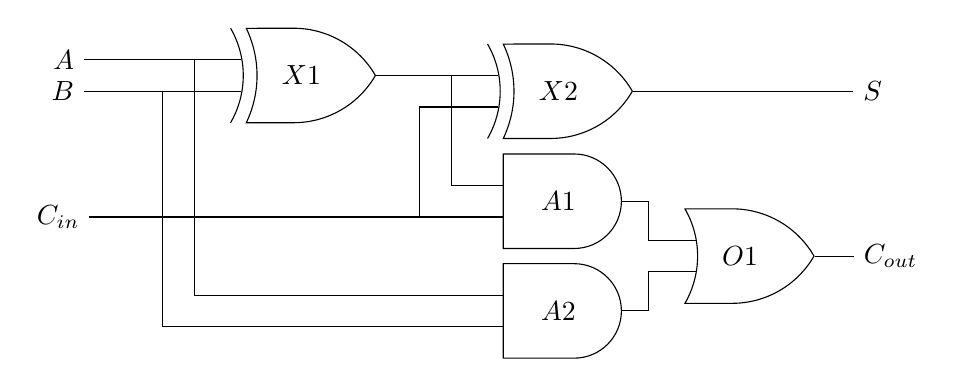
\begin{tikzpicture}[circuit logic US,
                    tiny circuit symbols,
                    every circuit symbol/.style={fill=white,draw,logic gate input sep=4mm, logic gate inverted radius=1mm}
]

\node [xor gate, inputs = nn,info=center:$X2$] at (0,0) (xor2) {};
\node [xor gate, inputs = nn,info=center:$X1$] at ($(xor2.input 1)+(-2.5,0)$) (xor1) {};
\node [and gate, inputs = nn,info=center:$A1$] at ($(xor2.north)+(0,-2)$) (and1) {};
\node [and gate, inputs = nn,info=center:$A2$] at ($(and1.north)+(0,-2)$) (and2) {};
\node [or gate, inputs = nn,info=center:$O1$] at ($(and1.output)!0.50!(and2.output)+(1.5,0)$) (or1) {};
\draw (xor1.output) |- (xor2.input 1);
\draw (xor1.input 1) -- ++(left:20mm) node[left] (A) {$A$};
\draw (xor1.input 2) -- ++(left:20mm) node[left] (B) {$B$};
\draw (xor2.input 1) -- ++(left:6mm) |- (and1.input 1) {};
\draw (xor2.input 2) -- ++(left:10mm) |- (and1.input 2) {};
\draw (xor2.output) -- ++(right:28mm) node[right] (S){$S$};
\draw (xor1.input 1) -- ++(left:6mm) |- (and2.input 1) {};
\draw (xor1.input 2) -- ++(left:10mm) |- (and2.input 2) {};
\draw (or1.input 1) -- ++(left:6mm) |- (and1.output) {};
\draw (or1.input 2) -- ++(left:6mm) |- (and2.output) {};
\draw (or1.output) -- ++(right:5mm) node[right] {$C_{out}$};
%
\draw
    (and1.input 2)
    -- ++(left:52.5mm)
    node[left] (CIN) {$C_{in}$};

\end{tikzpicture}
\end{document}
